\section{Experiments} \label{sec:experiments}

Greedy algorithms are often straightforward to develop and implement,
which explains their popular use in practical applications, such as
Bayesian experimental design and Active Learning, as discussed in
\secref{sec:active-learning} (also see the excellent introduction of \citet{nowak09})
and Adaptive Stochastic Set Cover, e.g., for filter design in streaming databases as discussed in \secref{sec:stochastic-set-cover}.
Besides allowing us to prove approximation guarantees for such algorithms, \term submodularity provides the following immediate practical benefits:
\begin{OneLiners}
\item[1.]  The ability to use lazy evaluations to speed up its execution.
\item [2.] The ability to generate data-dependent bounds on the optimal value. 
\end{OneLiners}
In this section, we empirically evaluate their benefits within a sensor selection application, in a setting similar to the one described by~\citet{vldb04}.  
In this application,  we have deployed a network $\sensors$ of wireless sensors, e.g., to monitor temperature in a building or traffic in a road network. Since sensors are battery constrained, we must adaptively select $k$ sensors, and then, given those sensor readings, predict, e.g., the temperature at all remaining locations.  This prediction is possible since temperature measurements will typically be correlated across space.  Here, we will consider the case where sensors can fail to report measurements due to hardware failures, environmental conditions or interference.


\subsection{The Sensor Selection Problem with Unreliable Sensors}

%
%
More formally, we imagine every location $\sensor\in\sensors$ is associated with a random variable $\cX_{\sensor}$ 
describing the temperature at that location, and there is a joint probability
distribution $\mass{\bx_{\sensors}} := \Pr{\cX_{\sensors} = \bx_{\sensors}}$ that models the correlation between temperature
values.  Here, $\cX_{\sensors}=[\cX_{1},\dots,\cX_{\numsensors}]$ is
the random vector over all temperature values. We follow \citet{vldb04} and assume that the joint distribution of the sensors is multivariate Gaussian.
A sensor $\sensor$ can make a noisy observation $\cY_{\sensor}=\cX_{\sensor}+\varepsilon_{\sensor}$, where $\varepsilon_{\sensor}$ is zero mean Gaussian noise with known variance $\sigma^{2}$.  
If some measurements $\cY_{A}=\by_{A}$ are obtained at a subset of locations, then the
conditional distribution
$\mass{\bx_{\sensors} \mid \by_{A}} := \Pr{\cX_{\sensors} =
    \bx_{\sensors} \mid\cY_{A}=\by_{A}}$ allows
predictions at the unobserved locations, e.g., by predicting
$\mathbb{E}[\cX_{\sensors}\mid\cY_{A}=\by_{A}]$ (which minimizes the mean squared error).
Furthermore, this conditional distribution quantifies the
\emph{uncertainty} in the prediction: Intuitively, we would like to
select sensors that minimize the predictive uncertainty.  One way to
quantify the predictive uncertainty is to use the remaining
Shannon entropy 
$$\entropy{ \cX_{\sensors}\mid\cY_{A} = \by_{A} }
:= \expct{-\log_2 \paren{\mass{ \cX_{\sensors}\mid \by_{A} }}}.$$

\noindent \looseness -1 We would like to adaptively select  $k$
sensors, to maximize the expected reduction in Shannon entropy (\cf~\citet{Sebastiani2000,KrauseG09}).  However, in practice, sensors are often unreliable, and might fail to report their measurements. We assume that after selecting a sensor, we find out whether it has failed or not 
before deciding which  sensor to select next.  We suppose that each sensor has an associated probability $\pfail{\sensor}$ of failure, in which case no reading is reported, and that sensor failures are independent of each other and of the ambient temperature at $\sensor$.
Thus we have an instance of the Stochastic Maximization problem with $\groundset := \sensors$, 
$\outcomes := \set{\text{working}, \text{failed}}$, and 
\begin{equation}
  \label{eq:exp-obj}
f(A, \rlz) := \entropy{ \cX_{\sensors}} - \entropy{ \cX_{\sensors}
 \  \mid \ \by_{ \set{  \sensor \ : \ \rlz(\sensor) = \text{working}  }  }   }  .
\end{equation}

\noindent For multivariate normal distributions, the entropy is given as
$$\entropy{ \cX_{\sensors}\mid\cY_{A} = \by_{A} }=\frac{1}{2}\ln (2\pi e)^{\numsensors}\left| \Sigma_{\sensors A}\left(\Sigma_{AA}+\sigma^{2} I\right)^{-1}\Sigma_{A \sensors}\right|,$$
where for sets $A$ and $B$, $\Sigma_{AB}$ denotes the covariance (matrix) between random vectors $\cX_{A}$ and $\cX_{B}$. Note that the predictive covariance does not depend on the actual observations $\by_{\cA}$, only on the set $A$ of chosen locations. Thus,
$$\entropy{ \cX_{\sensors}\mid\cY_{A} = \by_{A} } = \entropy{ \cX_{\sensors}\mid\cY_{A}},$$
where as usual, 
$\entropy{ \cX_{\sensors} \  \mid \ \cY_{A}} = \expct{ \entropy{
    \cX_{\sensors} \  \mid \ \cY_{A}= \by_A } }$.
As \citet{Krause05a} show, the function
\begin{equation}
  \label{eq:experiments-infogain}
  g(A) := \infogain{\cX_{\sensors}}{\cY_{A}}=\entropy{\cX_{\sensors}}-\entropy{\cX_{\sensors}\mid\cY_{A}}
\end{equation}
is monotone submodular, whenever the observations $\cY_{\sensors}$ are conditionally independent given $\cX_{\sensors}$.

This insight allows us to apply the result of
\secref{sec:stochastic-maximization} to show that the objective $f$ defined in~\eqnref{eq:exp-obj}
is adaptive monotone submodular, using 
$\hat{f}(S) := g(\set{\sensor : (\sensor, \text{working}) \in S})$ for
any $S \subseteq \groundset \times \outcomes$.


\subsubsection{Data and Experimental Setup}

Our first data set consists of temperature measurements from the network of $46$ sensors deployed at Intel Research Berkeley, which were sampled  at $30$ second intervals for $5$ consecutive days (starting Feb. $28^{\text{th}}$, $2004$). We define our objective function with respect to the empirical covariance estimated from the data.

We also use data from traffic sensors deployed along the highway I-$880$ South in California. We use traffic speed data for all working days from $6$ AM to $11$ AM for one month, from $357$ sensors. The goal is to predict the speed on all $357$ road segments. We again estimate the empirical covariance matrix.

\ignore{
All experiments were conducted using a Matlab R$2009$b
implementation of the adaptive greedy algorithms on a laptop with a
$2.26$ GHz Intel Core 2 Duo CPU and $4$ GB of DDR$3$ RAM.
} %


\subsubsection{The Benefits of Lazy Evaluation}
For both data sets, we run the adaptive greedy algorithm, using both the
naive implementation (\algref{alg:greedy}) and the accelerated version
using lazy evaluations (\algref{alg:acc-greedy}). We vary the
probability of sensor failure, 
and evaluate the execution time and the number of evaluations of the function $g$ (defined in
\eqnref{eq:experiments-infogain}) each algorithm makes.  
Figures~\ref{fig:berkeley-time} and~\ref{fig:traffic-time} plot
execution time given a $50\%$ sensor failure rate, on a computer with a
$2.26$ GHz dual core processor and $4$ GB RAM.  
In these applications, function evaluations are the bottleneck in the computation, so the
number of them serves as a machine-independent proxy for the running time. 
Figures~\ref{fig:berkeley-evals} and~\ref{fig:traffic-evals} show the
performance ratio in terms of this proxy. 
%
On the temperature data set, lazy evaluations speed up the computation
by a factor of between roughly $3.5$ and $7$, depending on the failure
probability.  On the larger traffic data set, we obtain speedup factors
between $30$ and $38$.
We find that the benefit of the lazy evaluations
increases with the problem size and with the
failure probability.  
The dependence on problem size must ultimately be explained in terms
of structural properties of the instances,
which also benefit the nonadaptive accelerated greedy algorithm.
The dependence on failure probability has a simpler explanation.
Note that in these applications, if the accelerated greedy algorithm selects $\sensor$, which then 
fails, then it does not need to make any additional function evaluations to select the
next sensor.  Contrast this with the naive greedy algorithm, which 
makes a function evaluation for each sensor that has not been selected
so far.  

\subsubsection{The Benefits of the Data Dependent Bound}
While \term submodularity allows us to prove worst-case performance
guarantees for the adaptive greedy algorithm, in many practical
applications it can be expected that these bounds are quite loose.
For our sensor selection application, we use the data dependent
bounds of \lemref{lem:rate-equation} to compute an upper bound
$\avgbound$ on $\max_{\policy} \avgf(\prune{\policy}{k})$ as described below,
and compare it with the performance guarantee
of~\thmref{thm:max-cover}. 
%
For the accelerated greedy algorithm, we use the upper bounds on the
marginal benefits stored in the priority queue instead of recomputing
the marginal benefits, and thus expect somewhat looser bounds. We find
that for our application, the bounds are tighter than the worst
case bounds. We also find that the ``lazy'' data dependent bounds are
almost as tight as the ``eager'' bounds using the 
eagerly recomputed marginal benefits $\diff{\prlz}{\elem}$  for the latest and
greatest $\prlz$, though the former have slightly higher variance.  
Figures~\ref{fig:berkeley-rewards} and~\ref{fig:traffic-rewards} show the
performance of the greedy algorithm as well as the three bounds on the
optimal value.


Two subtleties arise when using the data-dependent bounds 
to bound $\max_{\policy} \avgf(\prune{\policy}{k})$.
The first is that \lemref{lem:rate-equation} tells us that  
$\diff{\prlz}{\prune{\policy^*}{k}} \ \le \ \max_{A \subseteq \groundset, |A| \le
  k} \ \sum_{e \in A} \diff{\prlz}{e}$, whereas we would like to bound
the difference between
the optimal reward and 
the algorithm's current expected reward, conditioned on seeing
$\prlz$, i.e., $\expct{f(\played{\prune{\policy^*}{k}}{\rvrlz}, \rvrlz)  -
  f(\dom(\prlz), \rvrlz) \ \mid \ \rvrlz \sim \prlz  }$.
However, in our applications $f$ is strongly \term monotone, and strong
\term monotonicity implies that for any $\policy^*$ we have 
\begin{equation}
  \label{eq:experiments1}
  \expct{f(\played{\prune{\policy^*}{k}}{\rvrlz}, \rvrlz)  -
  f(\dom(\prlz), \rvrlz) \ \mid \ \rvrlz \sim \prlz  } \le \diff{\prlz}{\prune{\policy^*}{k}}. 
\end{equation}
Hence, if we let $\OPT(\prlz) := \max_{\policy}
\expct{f(\played{\prune{\policy}{k}}{\rvrlz}, \rvrlz) \ \mid \ \rvrlz \sim
  \prlz}$, 
 \lemref{lem:rate-equation} implies that 
\begin{equation}
  \label{eq:experiments2}
 \OPT(\prlz)  \le  \expct{f(\dom(\prlz), \rvrlz) \ \mid \ \rvrlz \sim
   \prlz} + \max_{A \subseteq \groundset, |A| \le
  k} \ \sum_{e \in A} \diff{\prlz}{e}. 
\end{equation}
 

The second subtlety is that we obtain a sequence of bounds from
\eqnref{eq:experiments2}.
If we consider the (random) sequence of partial realizations observed by the adaptive
greedy algorithm, $\emptyset = \prlz_0 \subset \prlz_1 \subset \cdots
\subset \prlz_k$, we obtain $k+1$ bounds $\bound_0, \ldots,
\bound_{k}$, where 
$\bound_{i} :=  \expct{f(\dom(\prlz_i), \rvrlz) \ \mid \ \rvrlz \sim
   \prlz_i} + \max_{A \subseteq \groundset, |A| \le
  k} \ \sum_{e \in A} \diff{\prlz_i}{e}$.
Taking the expectation over $\rvrlz$, note that for any $\policy$, and
any $i$, 
$$\avgf(\prune{\policy}{k}) \le \expct{\OPT(\prlz_i)} \le \expct{\bound_i}.$$
Therefore for any $0 \le i \le k$ , $\bound_i$ is a random variable
whose \emph{expectation} is an upper bound on the optimal expected reward of
any policy.  At this point we may be tempted to use the minimum of
these, i.e., $\bound_{\min} := \min_i \set{\bound_i}$ as our ultimate bound.
However, a collection of random variables $X_0, \ldots, X_k$ with
$\expct{X_i} \ge \tau$ for all $i$ does not, in general, satisfy 
$\min_i \set{X_i} \ge \tau$.  While it is possible in our case, with its
independent sensor failures, to use concentration inequalities to bound 
$\min_i \set{\bound_i} - \min_i \set{\expct{\bound_i}}$ with high
probability, and thus add an appropriate term to obtain a true upper
bound from $\bound_{\min}$, we take a different approach;
we simply use the average bound 
$\avgbound := \frac{1}{k+1}\sum_{i=0}^{k} \bound_i$.
Of course, depending on the application, a particular bound $\bound_i$
(chosen independently of the sequence $ \prlz_0, \prlz_1, \ldots,
\prlz_k$) may be superior.
For example, if $g$ is modular, then $\bound_0$ is best, whereas if
$g$ exhibits strong diminishing returns, then bounds $\bound_i$ with
larger values of $i$ may be significantly tighter.



\newcommand{\figwidth}{0.40\textwidth}
\newcommand{\figheightA}{0.22\textwidth}
\newcommand{\figheightB}{0.24\textwidth}


\begin{figure*}%
\centering 
\subfigure[\emph{Temperature Data: Execution time (sec) for 
 the naive vs accelerated implementations of adaptive greedy
  vs.\ the budget $k$ on number of sensors selected, 
  when $\pfail{\sensor} = 0.5$ for all $\sensor$, plotted with standard errors.}]{
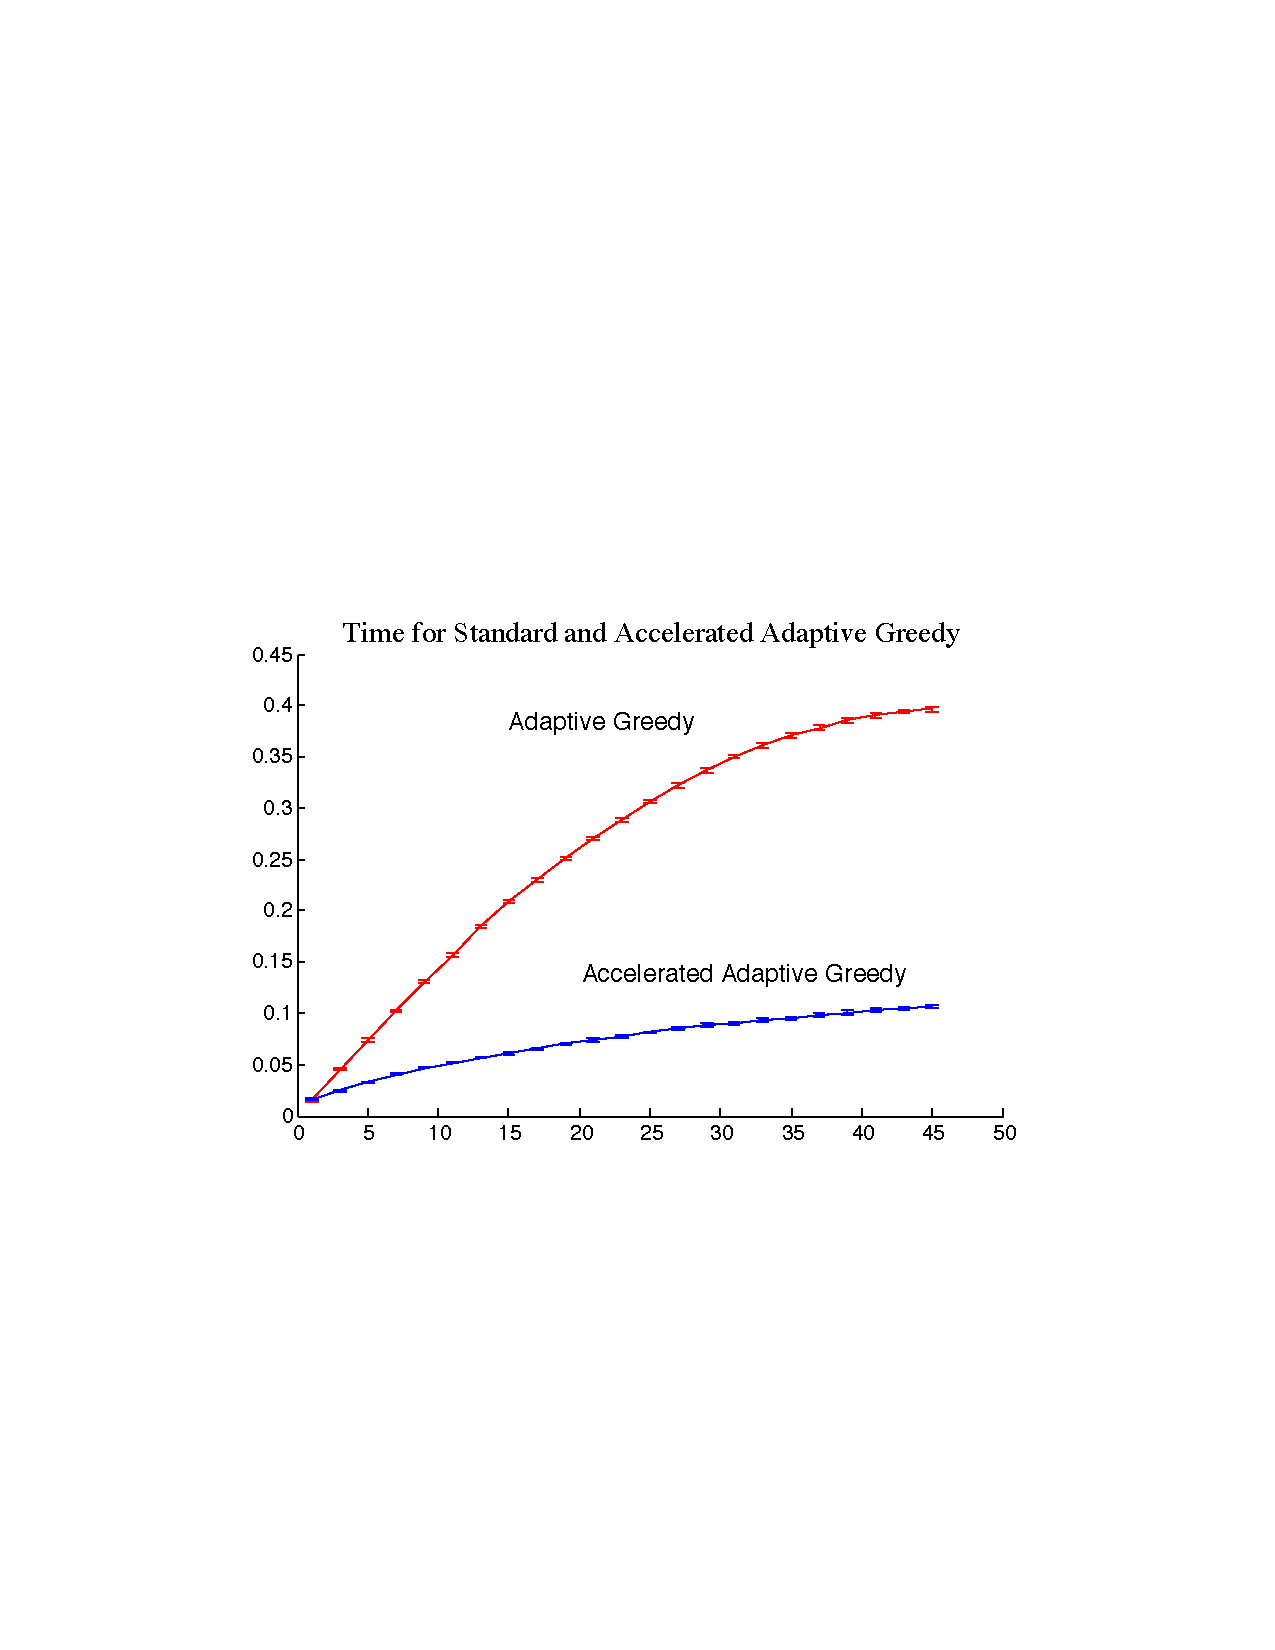
\includegraphics[width=\figwidth]{figs/berkeley_infogain_p50_n100_Time_shortfig_stderror} %
 \label{fig:berkeley-time}
}
\hspace{5mm}
\subfigure[\emph{Traffic Data: Execution time (sec) for 
 the naive vs accelerated implementations of adaptive greedy
  vs.\ the budget $k$ on number of sensors selected, 
  when $\pfail{\sensor} = 0.5$ for all $\sensor$, plotted with standard errors.}]{
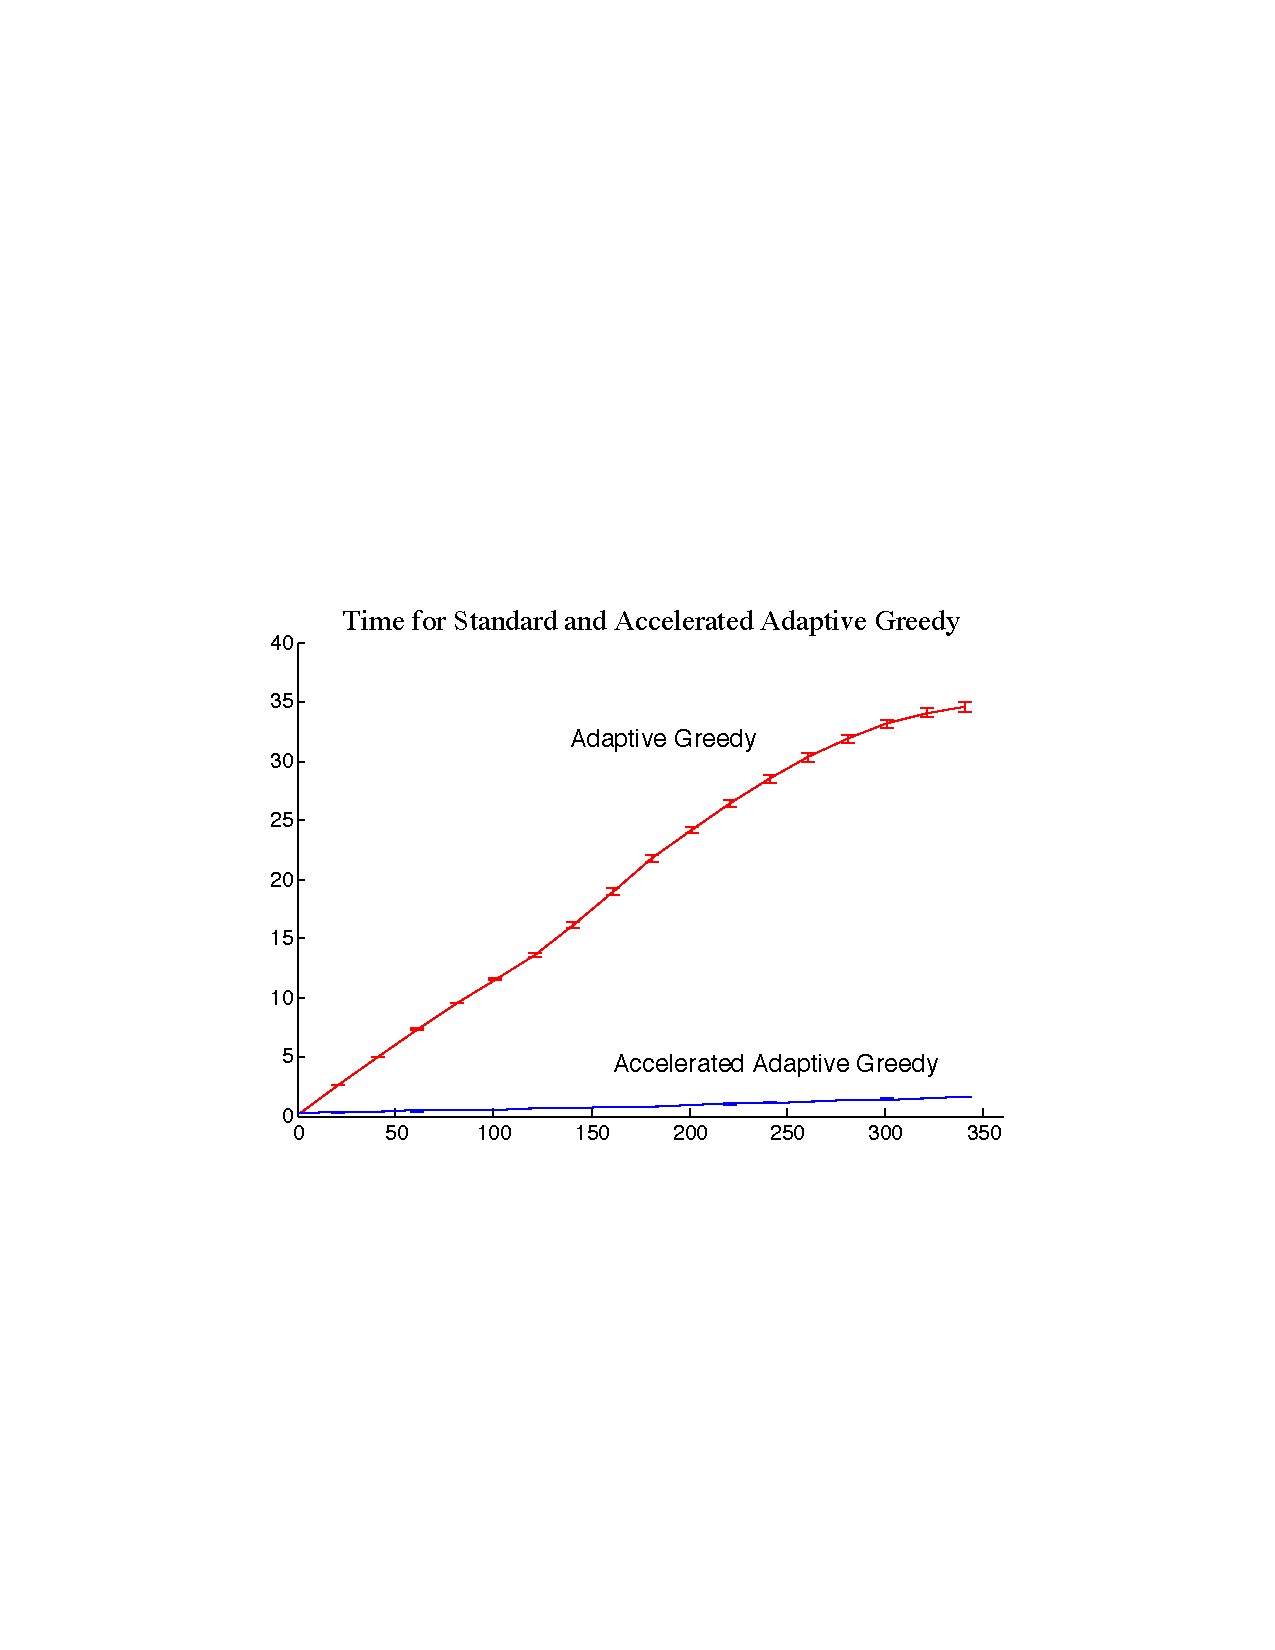
\includegraphics[width=0.38\textwidth]{figs/traffic_infogain_p50_n10_Time_shortfig_stderror}
 \label{fig:traffic-time}
}
\vspace{1mm}
\subfigure[\emph{Temperature Data: The ratio of function evaluations
  made by the naive vs accelerated implementations of adaptive greedy
  vs.\ the budget $k$ on number of sensors selected, for various
  failure rates.  Averaged over $100$ runs.}]{
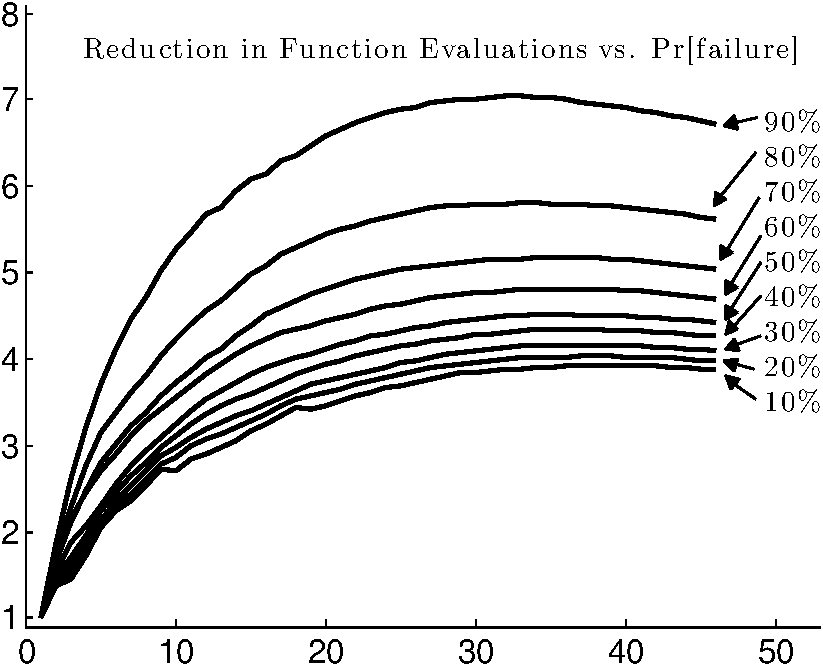
\includegraphics[width=\figwidth]{figs/berkeley_infogain_pVarious_n100_NevalsRatio}
 \label{fig:berkeley-evals}
 }
\hspace{5mm}
\subfigure[\emph{Traffic Data: The ratio of function evaluations
  made by the naive vs accelerated implementations of adaptive greedy
  vs.\ the budget $k$ on number of sensors selected, for various
  failure rates. Averaged over $10$ runs.}]{
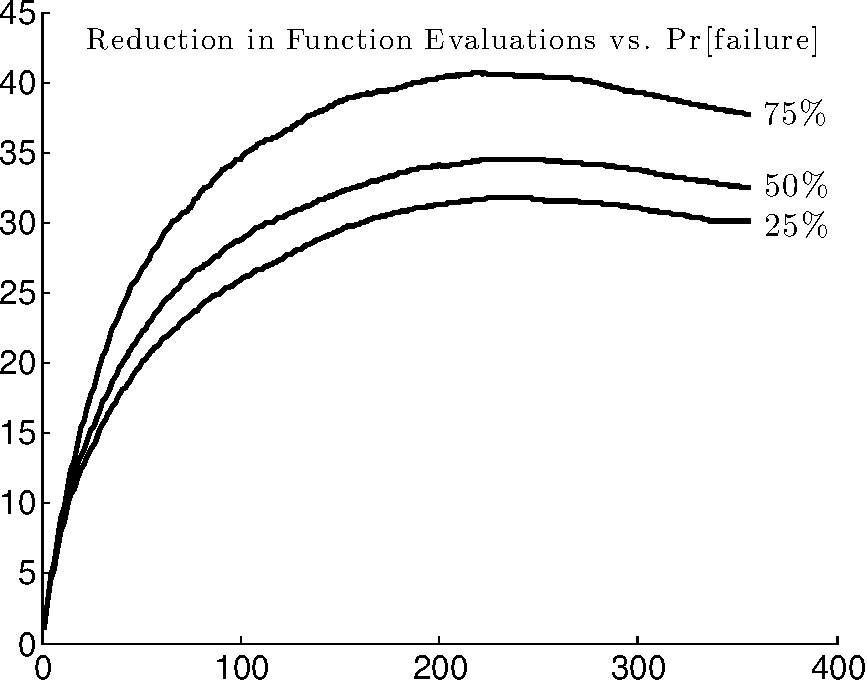
\includegraphics[width=\figwidth]{figs/traffic_infogain_pVarious_n10_NevalsRatio}
 \label{fig:traffic-evals}
}
\vspace{1mm}
\subfigure[\emph{Temperature Data: Rewards \& bounds on the \mbox{optimal} value when $\pfail{\sensor} = 0.5$ for
   all $\sensor$ vs.\ the budget $k$ on number of sensors
   selected, plotted with standard errors. %
}]{
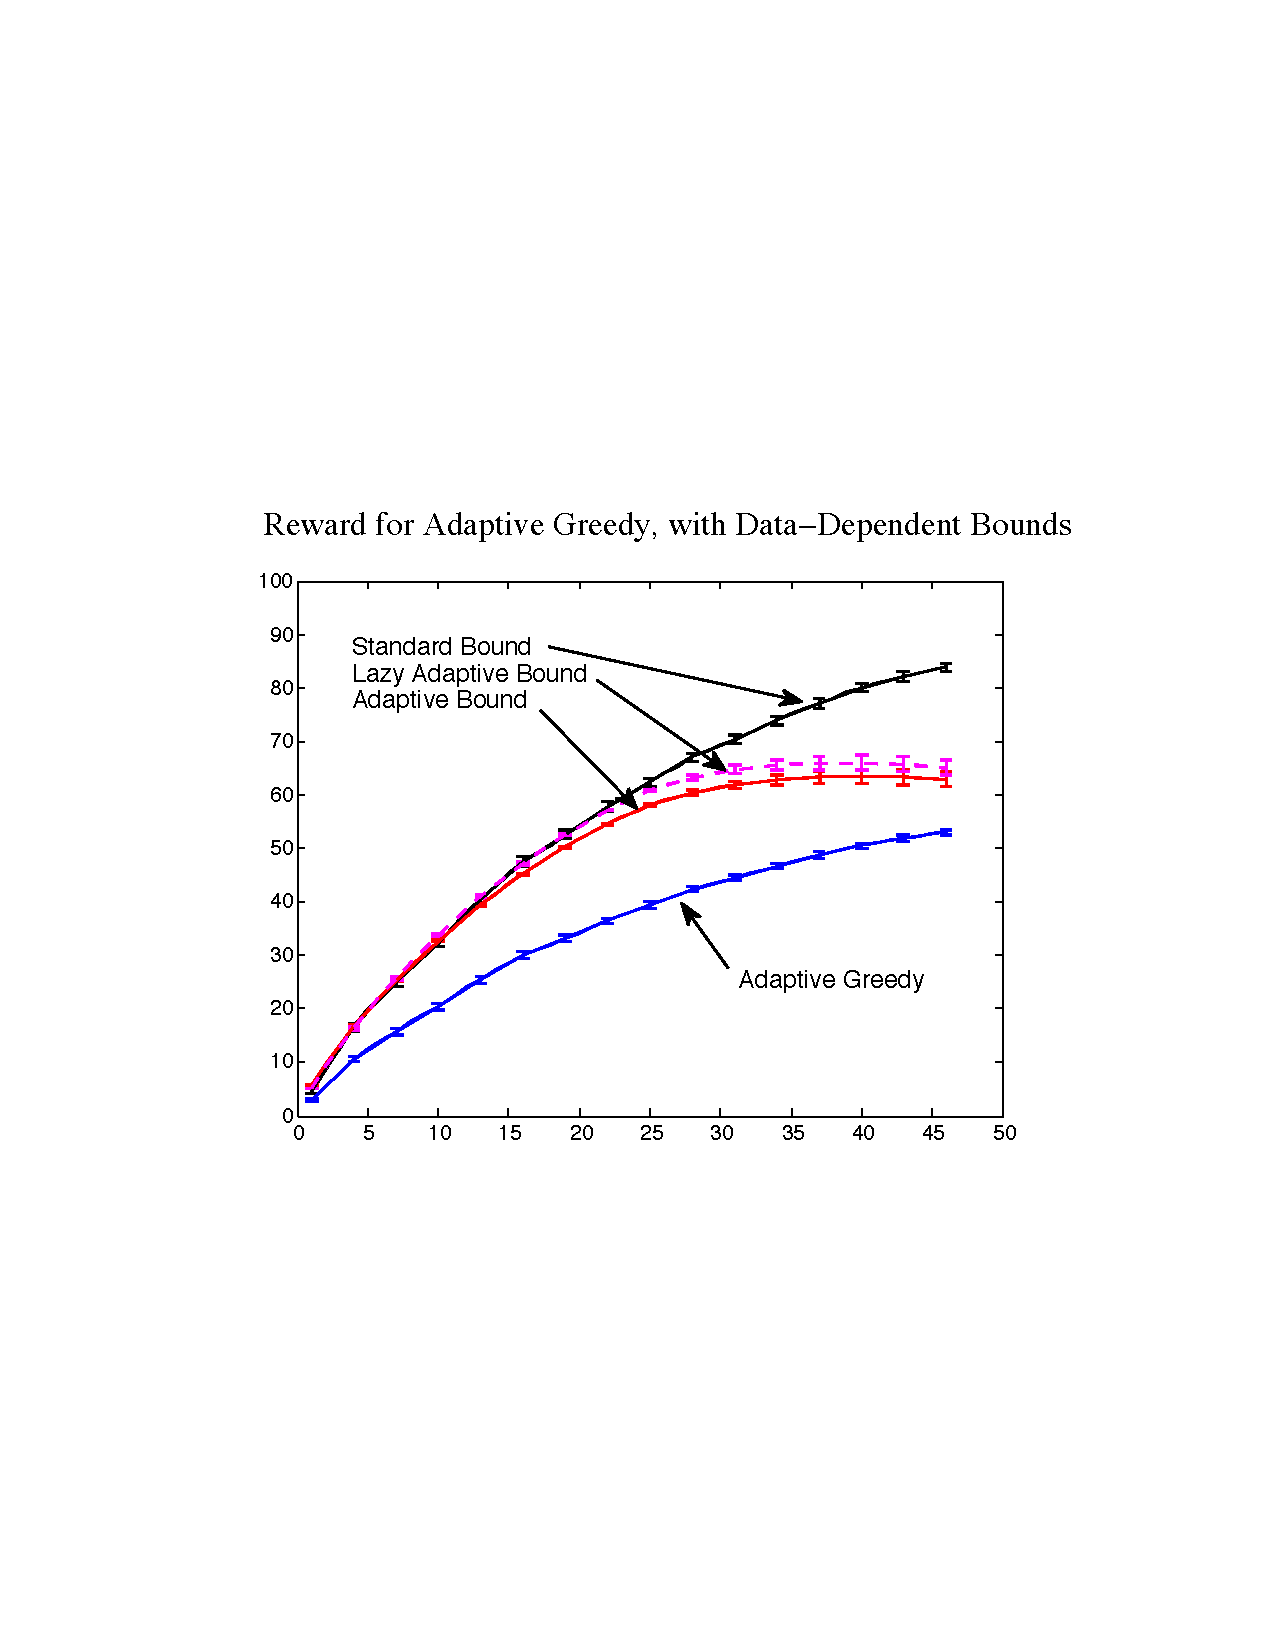
\includegraphics[width=\figwidth, height=2in]{figs/berkeley_infogain_p50_n100_Reward_errorbar_stderror}
 \label{fig:berkeley-rewards}
 }
\hspace{5mm}
\subfigure[\emph{Traffic Data: Rewards \& bounds on the optimal value when $\pfail{\sensor} = 0.5$ for
   all $\sensor$ vs.\ the budget $k$ on number of sensors
   selected, plotted with standard errors. %
}]{
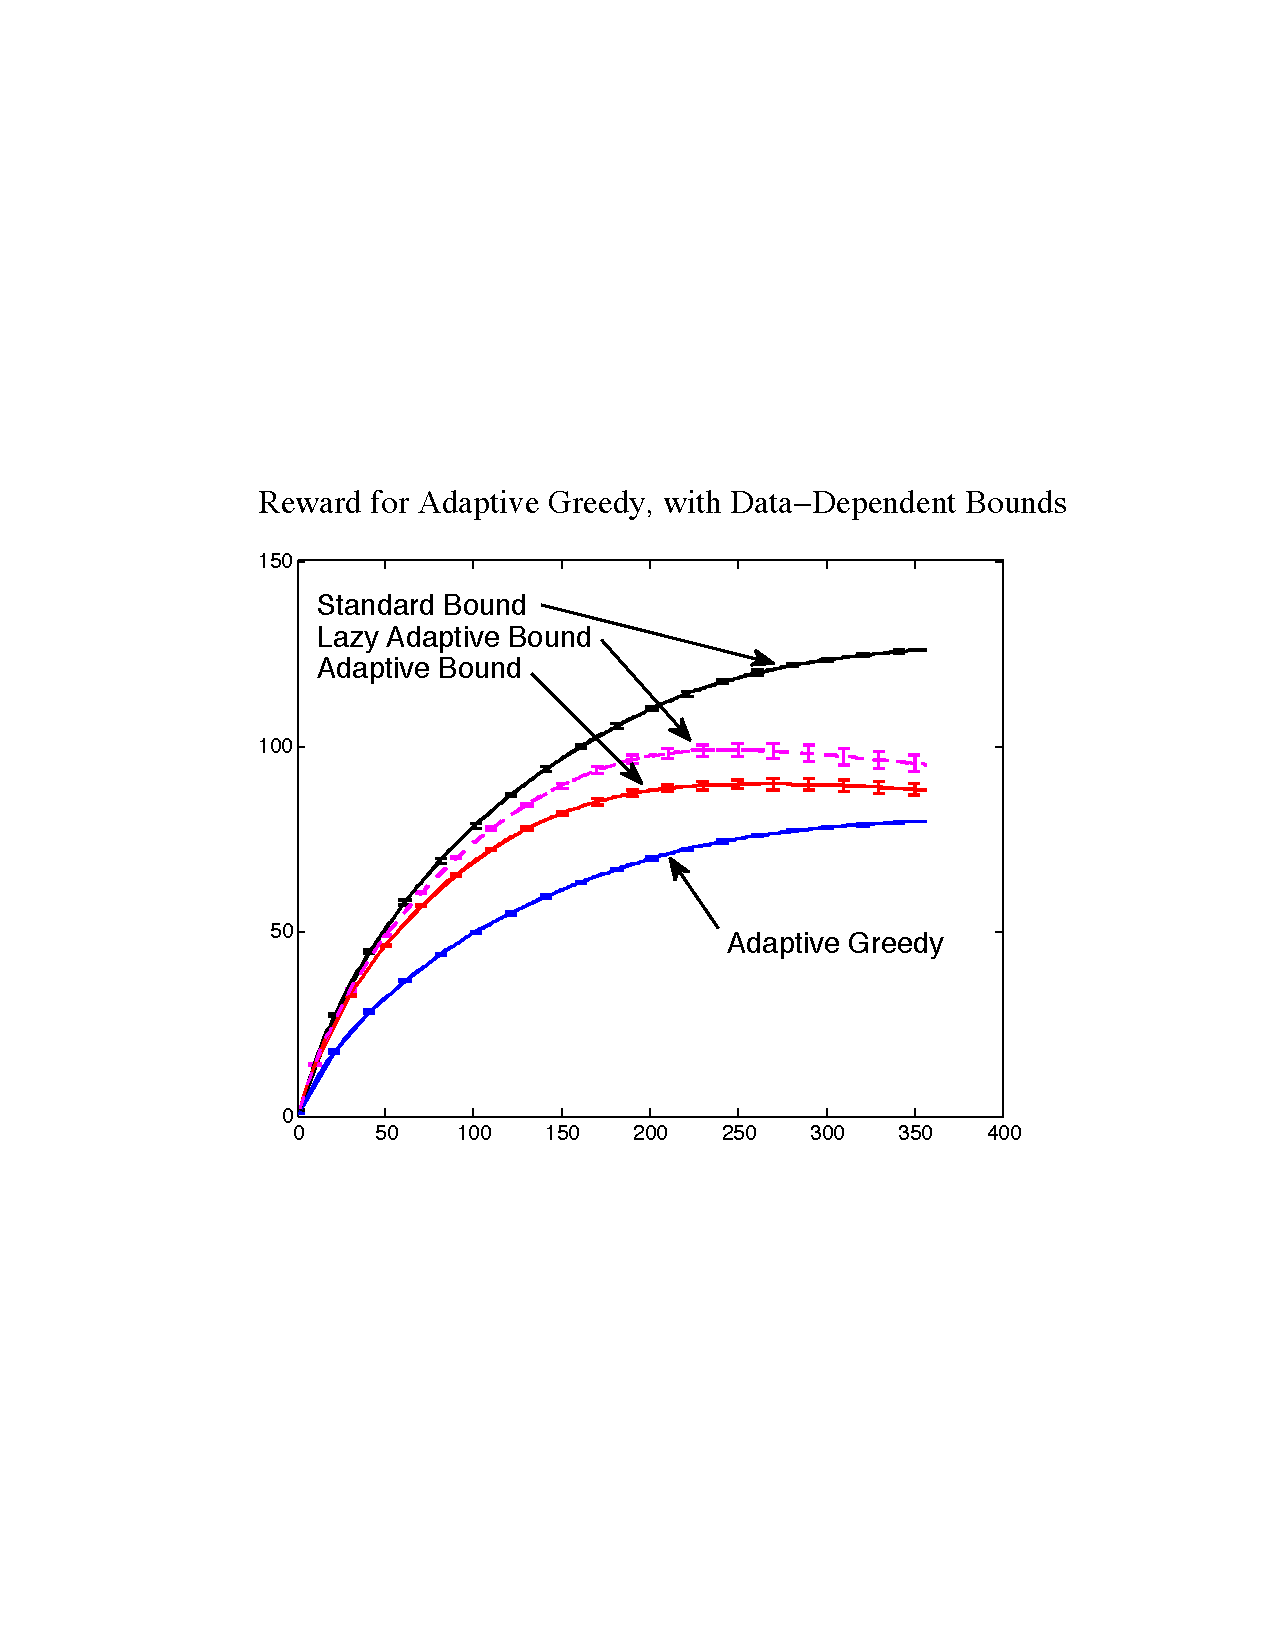
\includegraphics[width=\figwidth, height=2in]{figs/traffic_infogain_p50_n100_Reward_errorbar_stderror}
 \label{fig:traffic-rewards}
 }
\caption{%
Experimental results.  
\label{fig:experiments}
 }%
\end{figure*}






\ignore{
%
\begin{figure*}%
\centering 
\subfigure[\emph{Temperature Data: The ratio of function evaluations
  made by the naive vs accelerated implementations of adaptive greedy
  vs.\ the budget $k$ on number of sensors selected, for various
  failure rates.  Averaged over $100$ runs.}]{
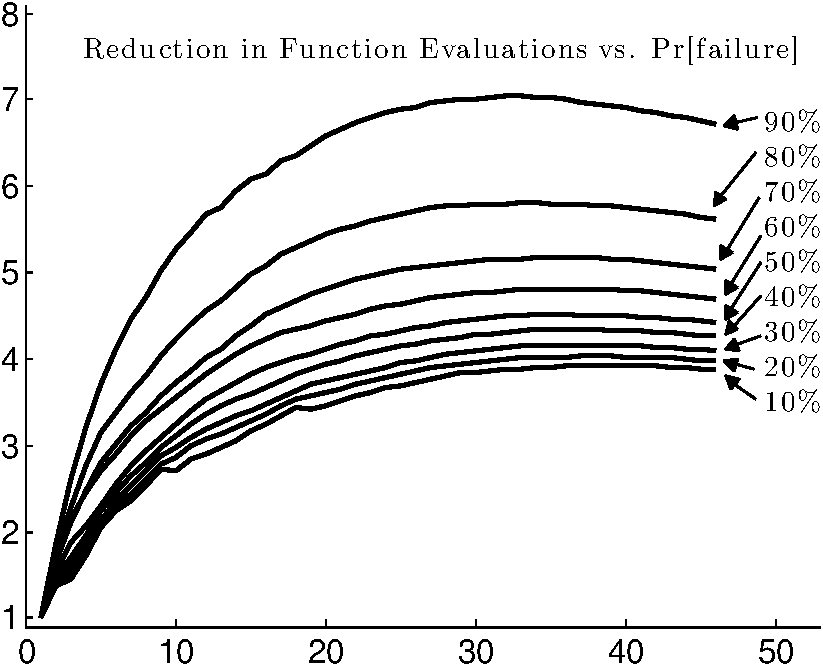
\includegraphics[width=\figwidth]{figs/berkeley_infogain_pVarious_n100_NevalsRatio}
 \label{fig:berkeley-evals}
 }
\hspace{5mm}
\subfigure[\emph{Temperature Data: Rewards \& bounds on the \mbox{optimal} value when $\pfail{\sensor} = 0.5$ for
   all $\sensor$ vs.\ the budget $k$ on number of sensors selected. Averaged over $100$ runs.}]{
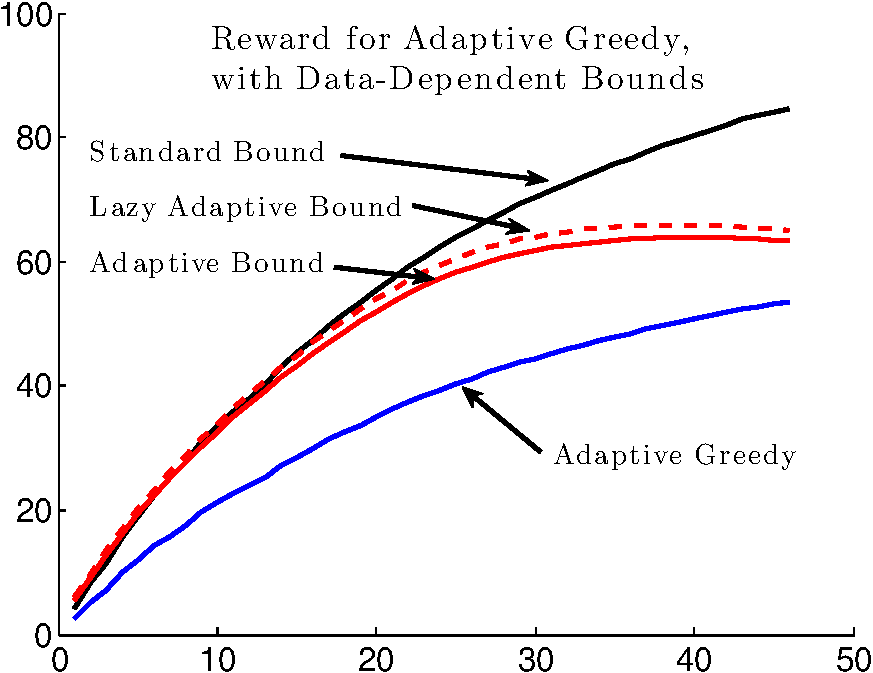
\includegraphics[width=\figwidth]{figs/berkeley_infogain_p50_n100_avgB}
 \label{fig:berkeley-rewards}
 }
\vspace{5mm}
\subfigure[\emph{Traffic Data: The ratio of function evaluations
  made by the naive vs accelerated implementations of adaptive greedy
  vs.\ the budget $k$ on number of sensors selected, for various
  failure rates. Averaged over $10$ runs.}]{
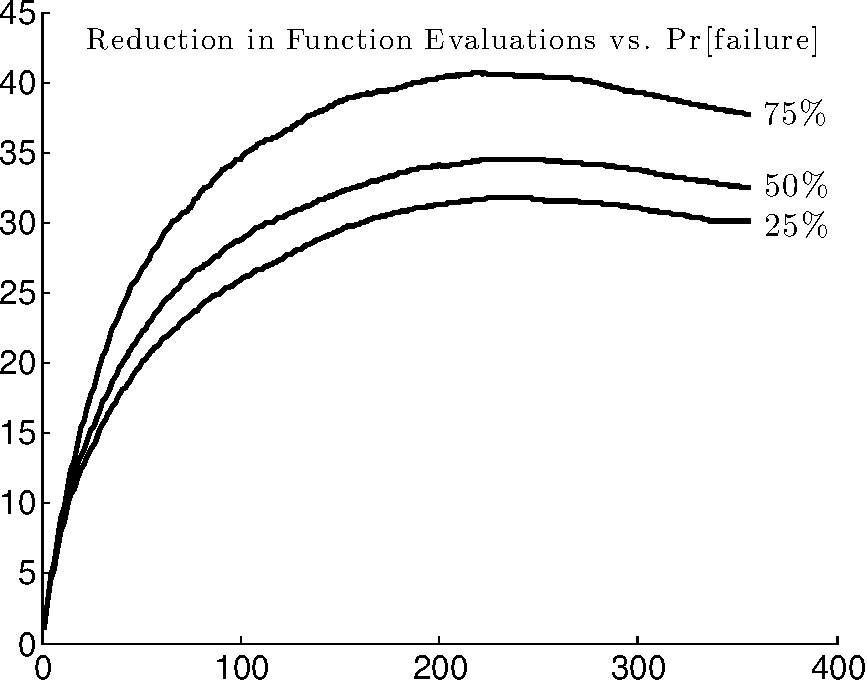
\includegraphics[width=\figwidth]{figs/traffic_infogain_pVarious_n10_NevalsRatio}
 \label{fig:traffic-evals}
}
\hspace{5mm}
\subfigure[\emph{Traffic Data: Rewards \& bounds on the optimal value when $\pfail{\sensor} = 0.5$ for
   all $\sensor$ vs.\ the budget $k$ on number of sensors selected. Averaged over $10$ runs.}]{
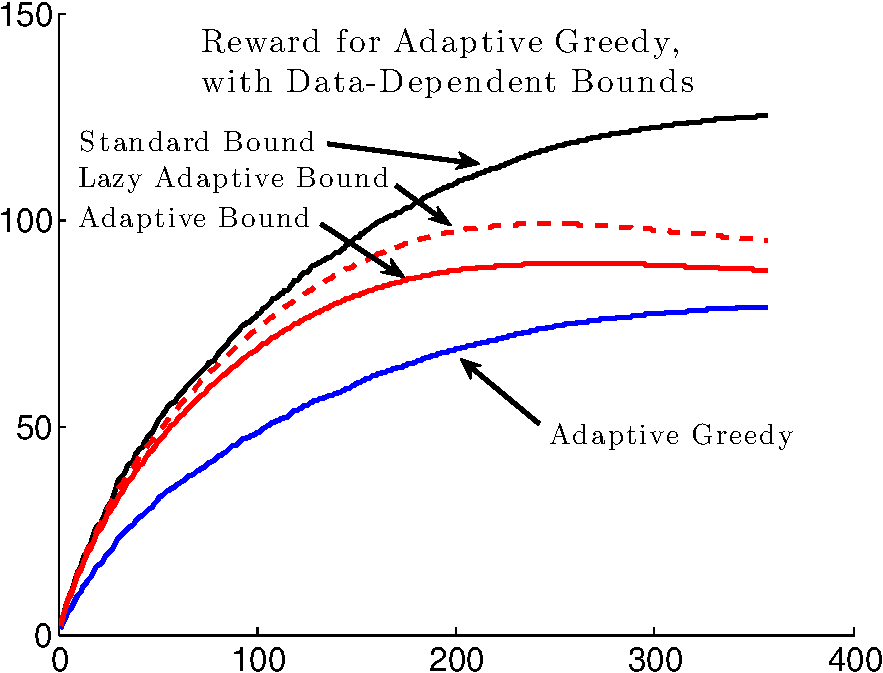
\includegraphics[width=\figwidth]{figs/traffic_infogain_p50_n10_noise25_avgB}
 \label{fig:traffic-rewards}
 }
\caption{%
Experimental results.  
\label{fig:experiments}
 }%
\end{figure*}
}

\ignore{
\begin{figure}[p]
\begin{minipage}[b]{0.5\linewidth}
\centering
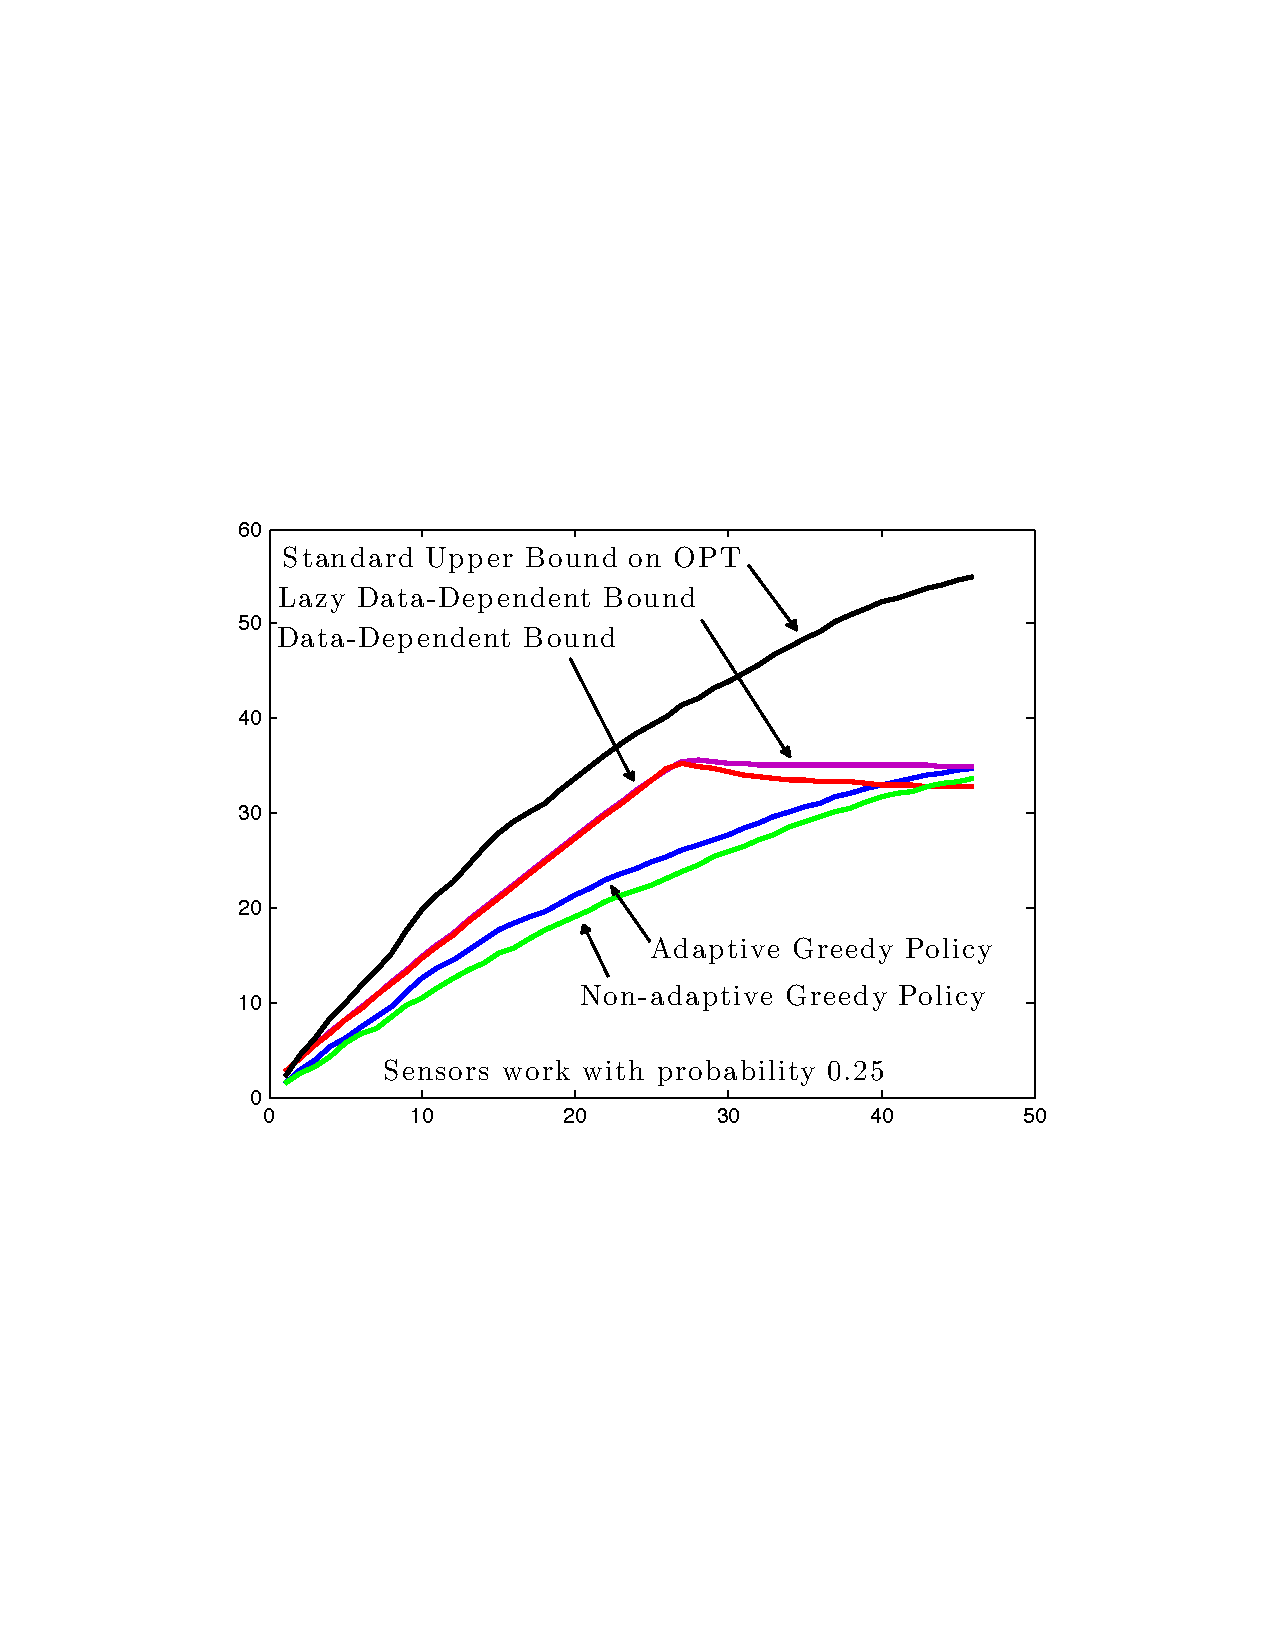
\includegraphics[width=1.0\textwidth, height=6cm]{figs/Berkeley_pwork25}
%
%
\end{minipage}
\hspace{0.5cm}
\begin{minipage}[b]{0.5\linewidth}
\centering
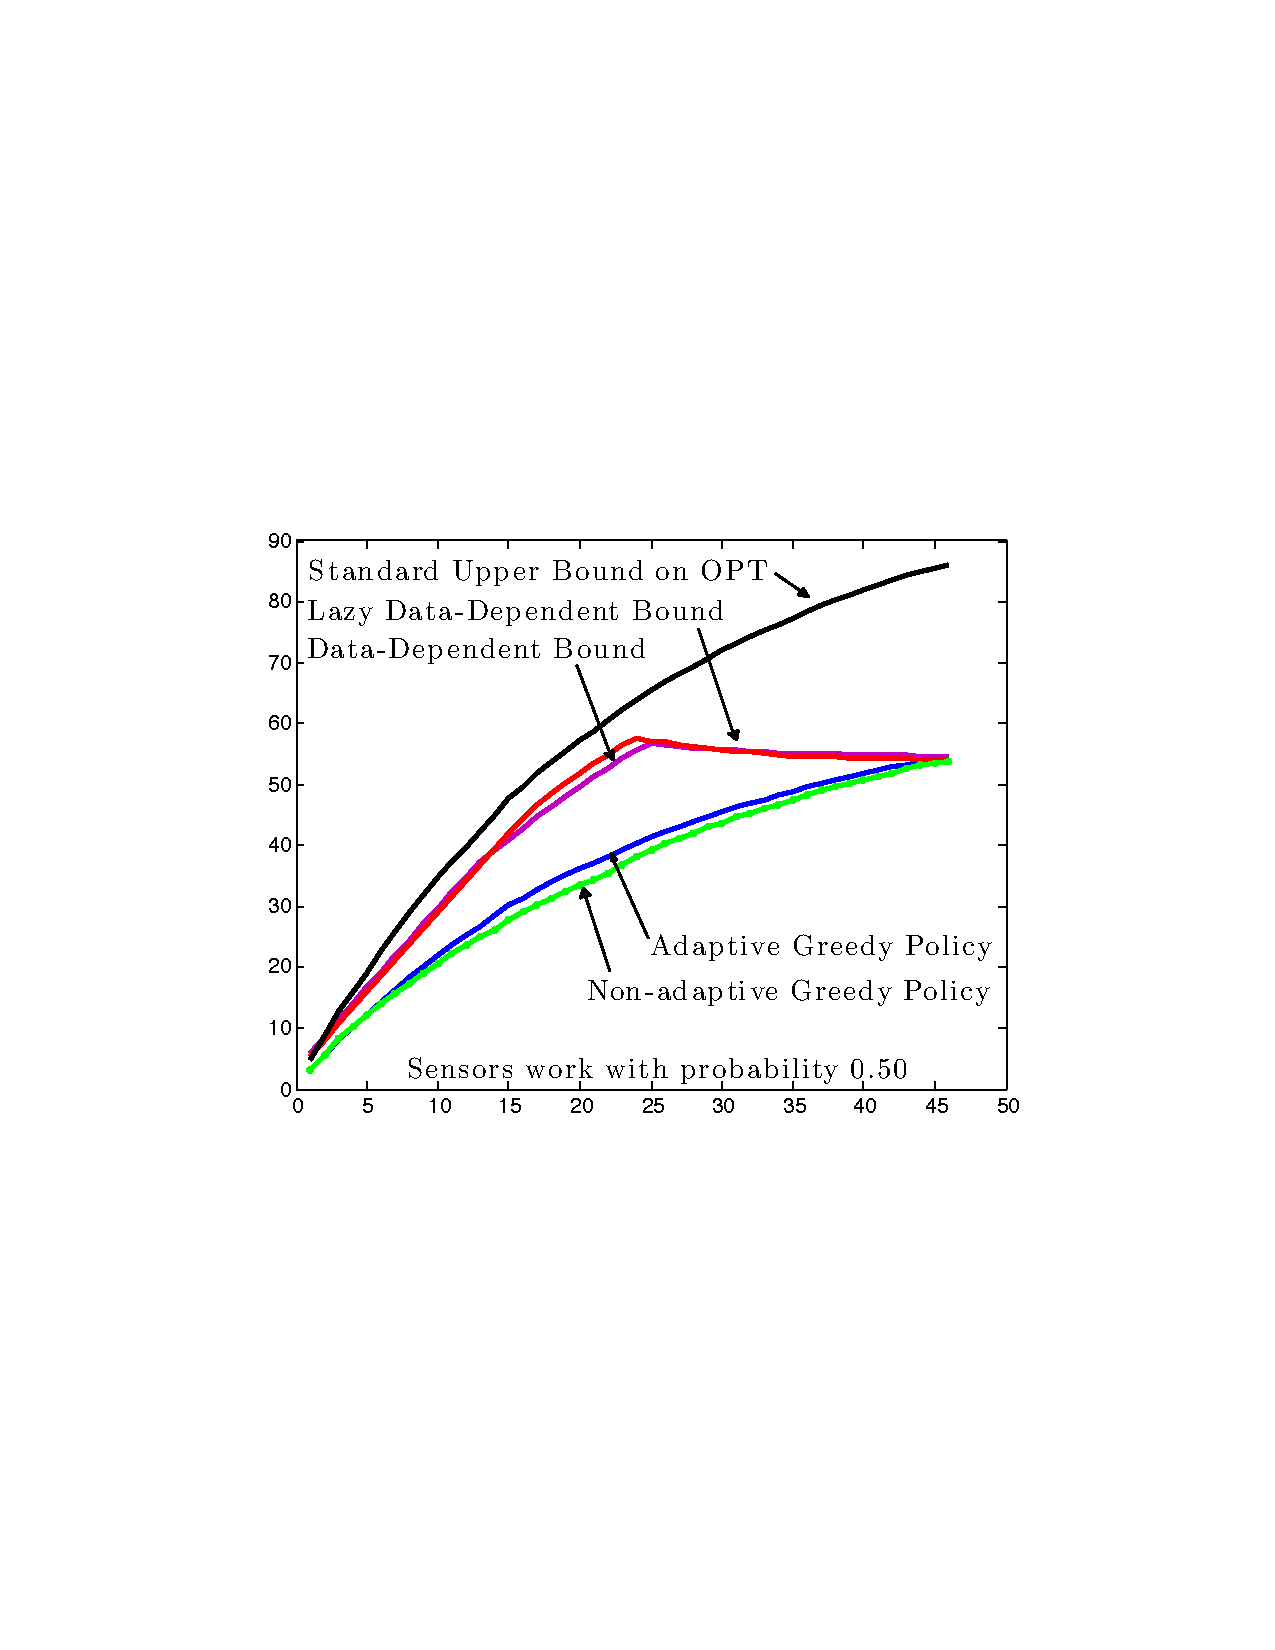
\includegraphics[width=1.0\textwidth, height=6cm]{figs/Berkeley_pwork50}
%
%
\end{minipage}\\
\begin{minipage}[b]{0.5\linewidth}
\centering
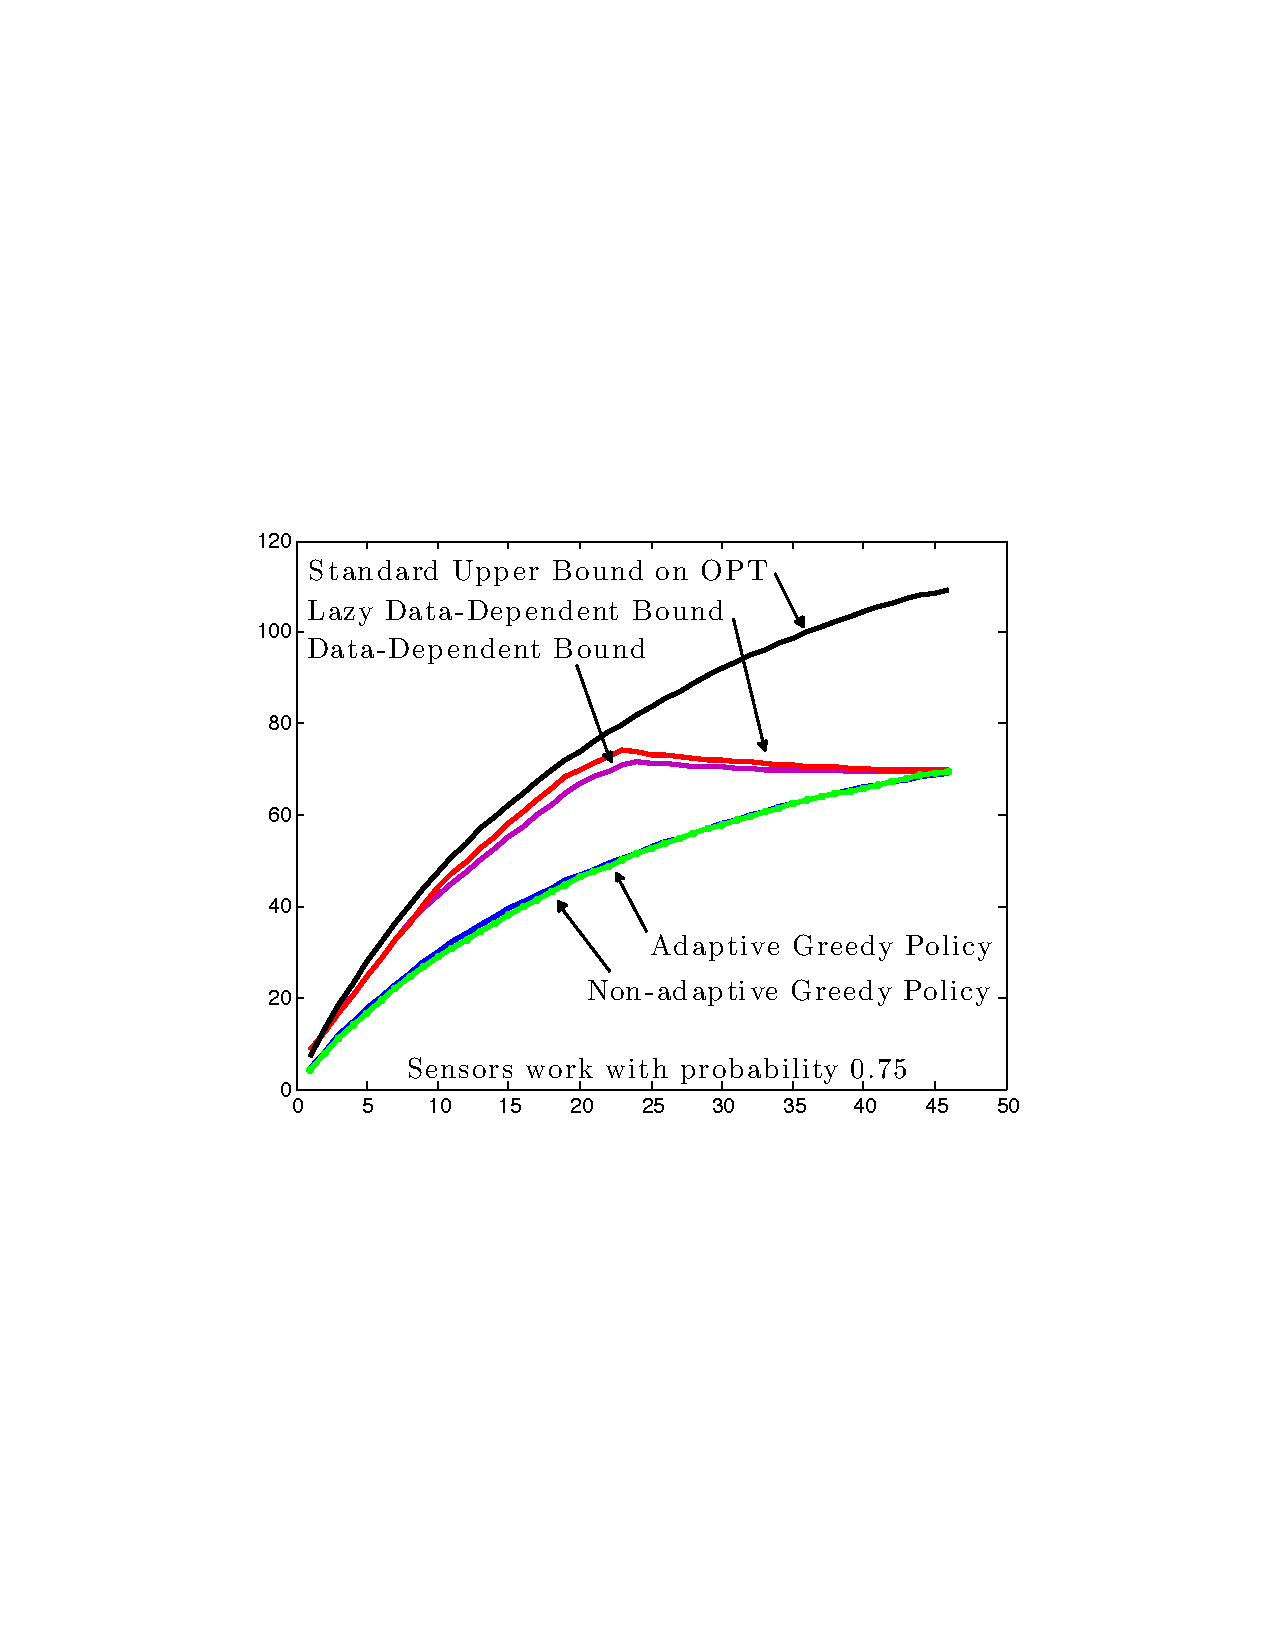
\includegraphics[width=1.0\textwidth, height=6cm]{figs/Berkeley_pwork75}
%
%
\end{minipage}
\hspace{0.5cm}
\begin{minipage}[b]{0.5\linewidth}
\centering
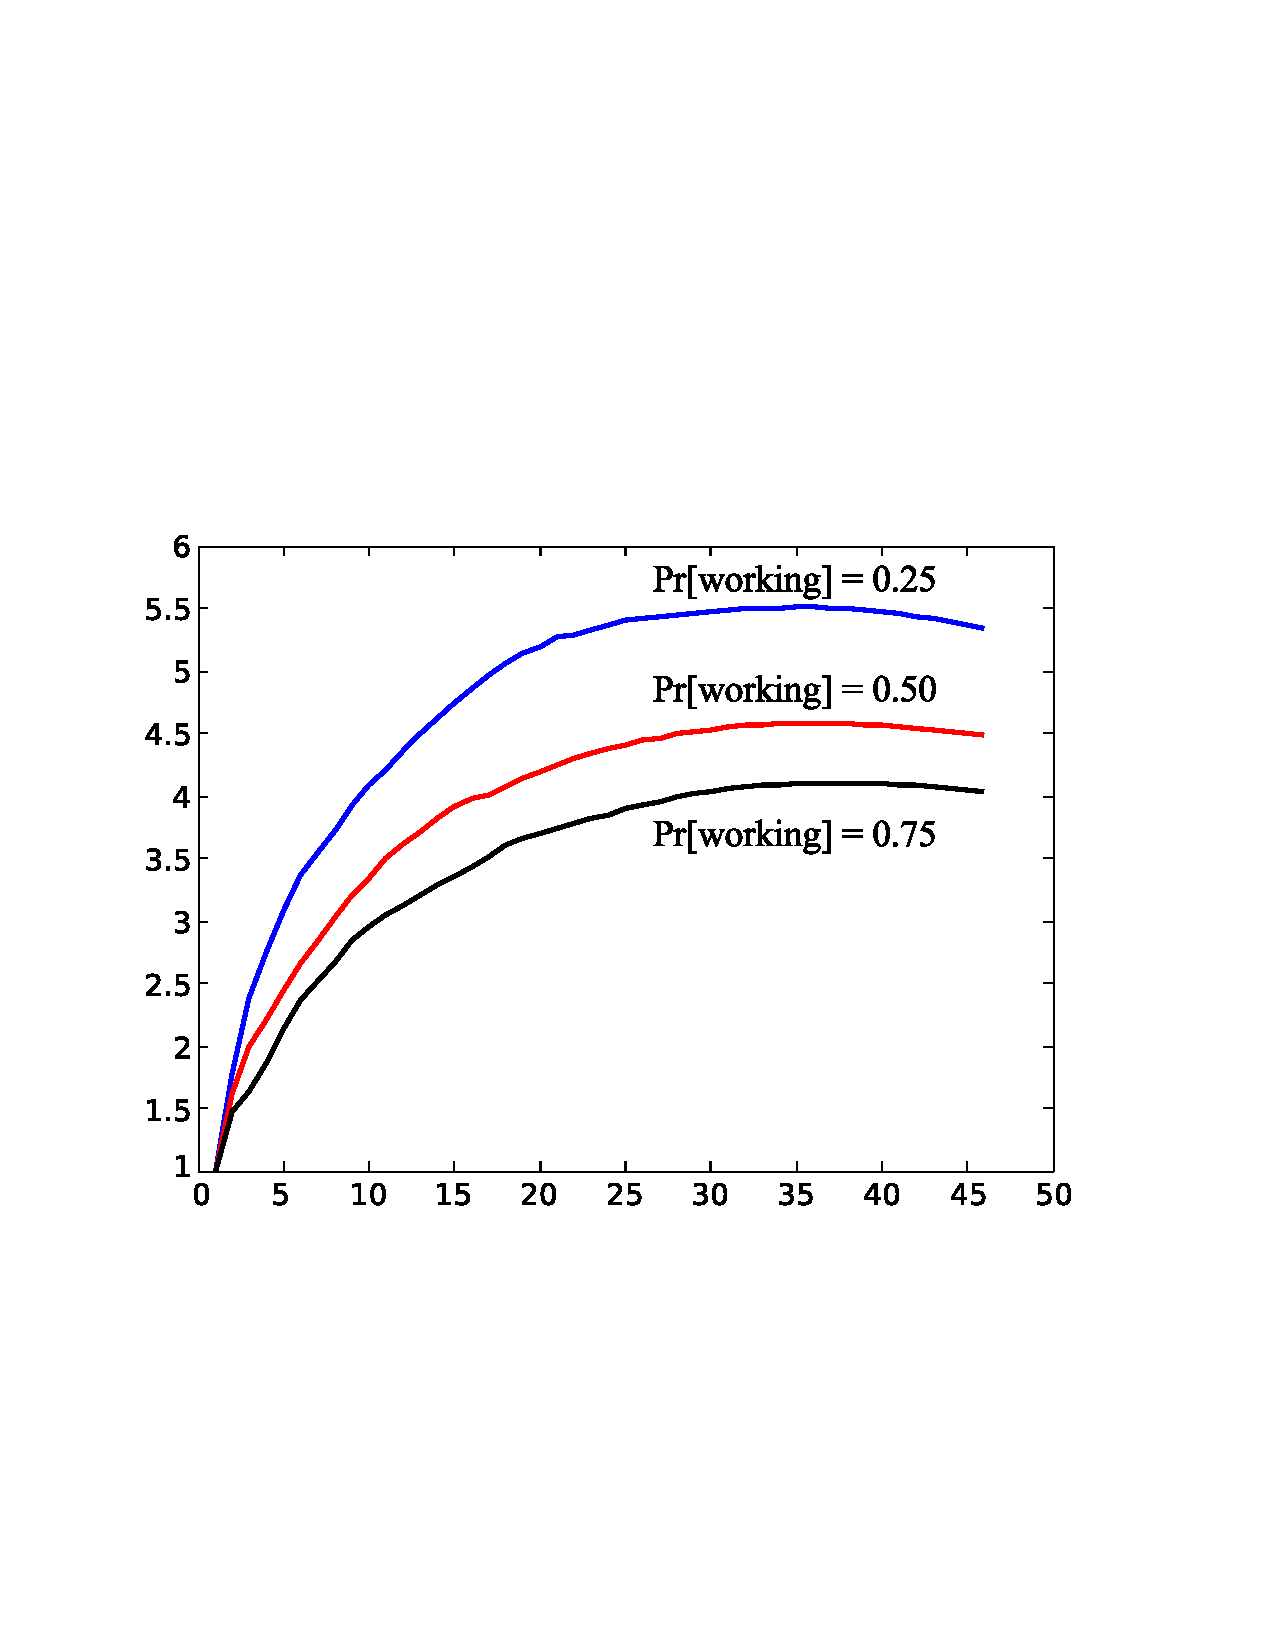
\includegraphics[width=1.0\textwidth, height=6cm]{figs/Berkeley_evals}
\end{minipage}
\caption{
Top-left, top-right, and bottom-left:
Reward vs. number of selected sensor locations, for
  independent probabilities of sensors working.  The standard upper
  bound is simply $e/(e-1)$ times the reward obtained.  Tighter upper
  bounds may be obtained from the data-dependent bounds using 
  the best available conditional expected marginal benefits in the
  priority queue (for the lazy bound), or using the current values
 (for the standard data dependent bound).  Finally, the reward of the
 adaptive and non-adaptive greedy policies are displayed.  
 These results are the average of $100$ trials.  Unfortunately,
 adaptivity does not appear to help much in this application, however
 on the positive side this contributes to the fact that the lazy data-dependent bounds
 are nearly as good as the standard ones, despite using many fewer
 function evaluations.
Bottom-right: Ratio of function evaluations made by the adaptive greedy
  algorithm and its accelerated (lazy) variant vs. the number of
  selected sensor locations,  for three different
  probabilities of sensors working. 
}
\label{fig:temp-data-rewards}
\end{figure}
} %



%
%
%
%
